% concluding thoughts

\chapter{Outlook}\label{ch:concl}

In the previous chapters we have described the XENON1T detector (Chapter~\ref{ch:xe1t}), two new calibration sources (Chapters~\ref{ch:ng} and~\ref{ch:rn220}), and an off-line analysis to reduce backgrounds from \Rn~(Chapter~\ref{ch:convection}).

\section{Neutron Generator}

While the first NR calibration on XENON1T was done using $^{241}$AmBe~\cite{Aprile:2017iyp}, this was due to technical issues with the neutron generator. The activity of the $^{241}$AmBe source approved for use at LNGS is not very high, leading one analysis coordinator to quip that the NR calibration data collected with it was merely background data with NR contamination. Further, The low-energy neutrons emitted by $^{241}$AmBe thermalize quickly and are absorbed in the water between the source and the outer cryostat, resulting in a not inconsiderable rate of the $2.2\1{MeV}$ line from capture on $^{1}$H. The neutron generator is not exempt from this, but the lack of low-energy neutrons means fewer neutrons thermalize in the immediate vacinity of the source. Additionally, the adjustable neutron production rate allows the detector to be calibrated at the maximum rate allowed by the DAQ, minimizing the necessary calibration time. Finally, the quasi-monoenergetic neutron spectrum from the neutron generator allows for accurate \textit{in-situ} measurements of the light and charge yield as reported by LUX~\cite{Akerib:2016mzi}.

\section{$^{220}$Rn source}

The $^{220}$Rn source was designed for use on detectors at the tonne scale or larger where calibration from external sources is impractical or impossible. It has been deployed on XENON1T a total of 8 times with a combined runtime of over 30 days. These data are primarily used to characterize the low-energy electronic recoil band, utilizing decays of $^{212}$Pb. As leakage from the ER band into the NR band is the dominant source of events in the NR signal region~\cite{Aprile:2015uzo}, the characterization of this signal region is of the utmost importance. $\n{CH_3T}$ was deployed on XENON100~\cite{Aprile:2017xxh}, but the removal of the introduced activity was not as straightforward as expected from the LUX calibration with the same~\cite{Akerib:2015wdi}. Though this calibration was performed at the end of the operation of XENON100 and thus did not impact its sensitivity, with even a remote possiblity of a similar outcome for XENON1T the decision was made to use $^{220}$Rn and not $\n{CH_3T}$.

Furthermore, this source will be used on the next-generation ($\order{10}~tonne$) XENONnT and LZ~\cite{Akerib:2018lyp,Mount:2017qzi} experiments, scheduled to enter operation in 2018 and 2019, with science data anticipated in the following years. This source is also expected to be used in the 50~tonne DARWIN experiment~\cite{Aalbers:2016jon}, anticipated for 2025.

\section{Radon backgrounds in future detectors}

The LZ and XENONnT detectors are expected to be capable of probing a spin-independent WIMP-nucleon scattering cross section of $10^{-48}\1{cm^2}$. As the sensitivity is largely limited by the \Rn~based backgrounds, new methods are required to achieve the necessary radon concentration of $\sim1\1{mBq/tonne}$. Traditionally, the method of radon background reduction was by using materials with lower uranium contaminations~\cite{Aprile:2017ilq,Akerib:2017iwt}. XENON100 demonstrated how cryogenic distillation could be used to reduce the radon concentration during detector operation~\cite{Aprile:2017kop}, and XENONnT will have a distillation column dedicated for online radon removal. While online distillation can be implemented after a detector enters operation, unless the recirculation system is designed to work in conjuction with such a column, the benefits are typically limited.

In Chapter~\ref{ch:convection} we discussed the radon veto, a fundamentally new method of radon background removal. This technique has the distinct advantage of being based on data analysis rather than hardware, and thus can be done even after a detector has ended operations. However, it does cost some exposure which hardware-based methods do not. What remains to be investigated is how a detector's design can be optimized to facilitate the radon veto analysis.

\section{On the horizon}

Looming some years away is the DARWIN project~\cite{Aalbers:2016jon}, featuring a total of 50~tonnes of xenon. This represents the endpoint of the liquid xenon dark matter detector, capable of probing a WIMP-nucleon cross section of $10^{-49}\1{cm^2}$. While a larger detector could be constructed, as shown in Figure~\ref{fig:darwin_sens}, signals from coherent neutrino-nuclear scattering represent an unavoidable background of low-energy nuclear recoils, making a search to smaller cross-sections much more difficult.

\begin{figure}[htb]
\centering
    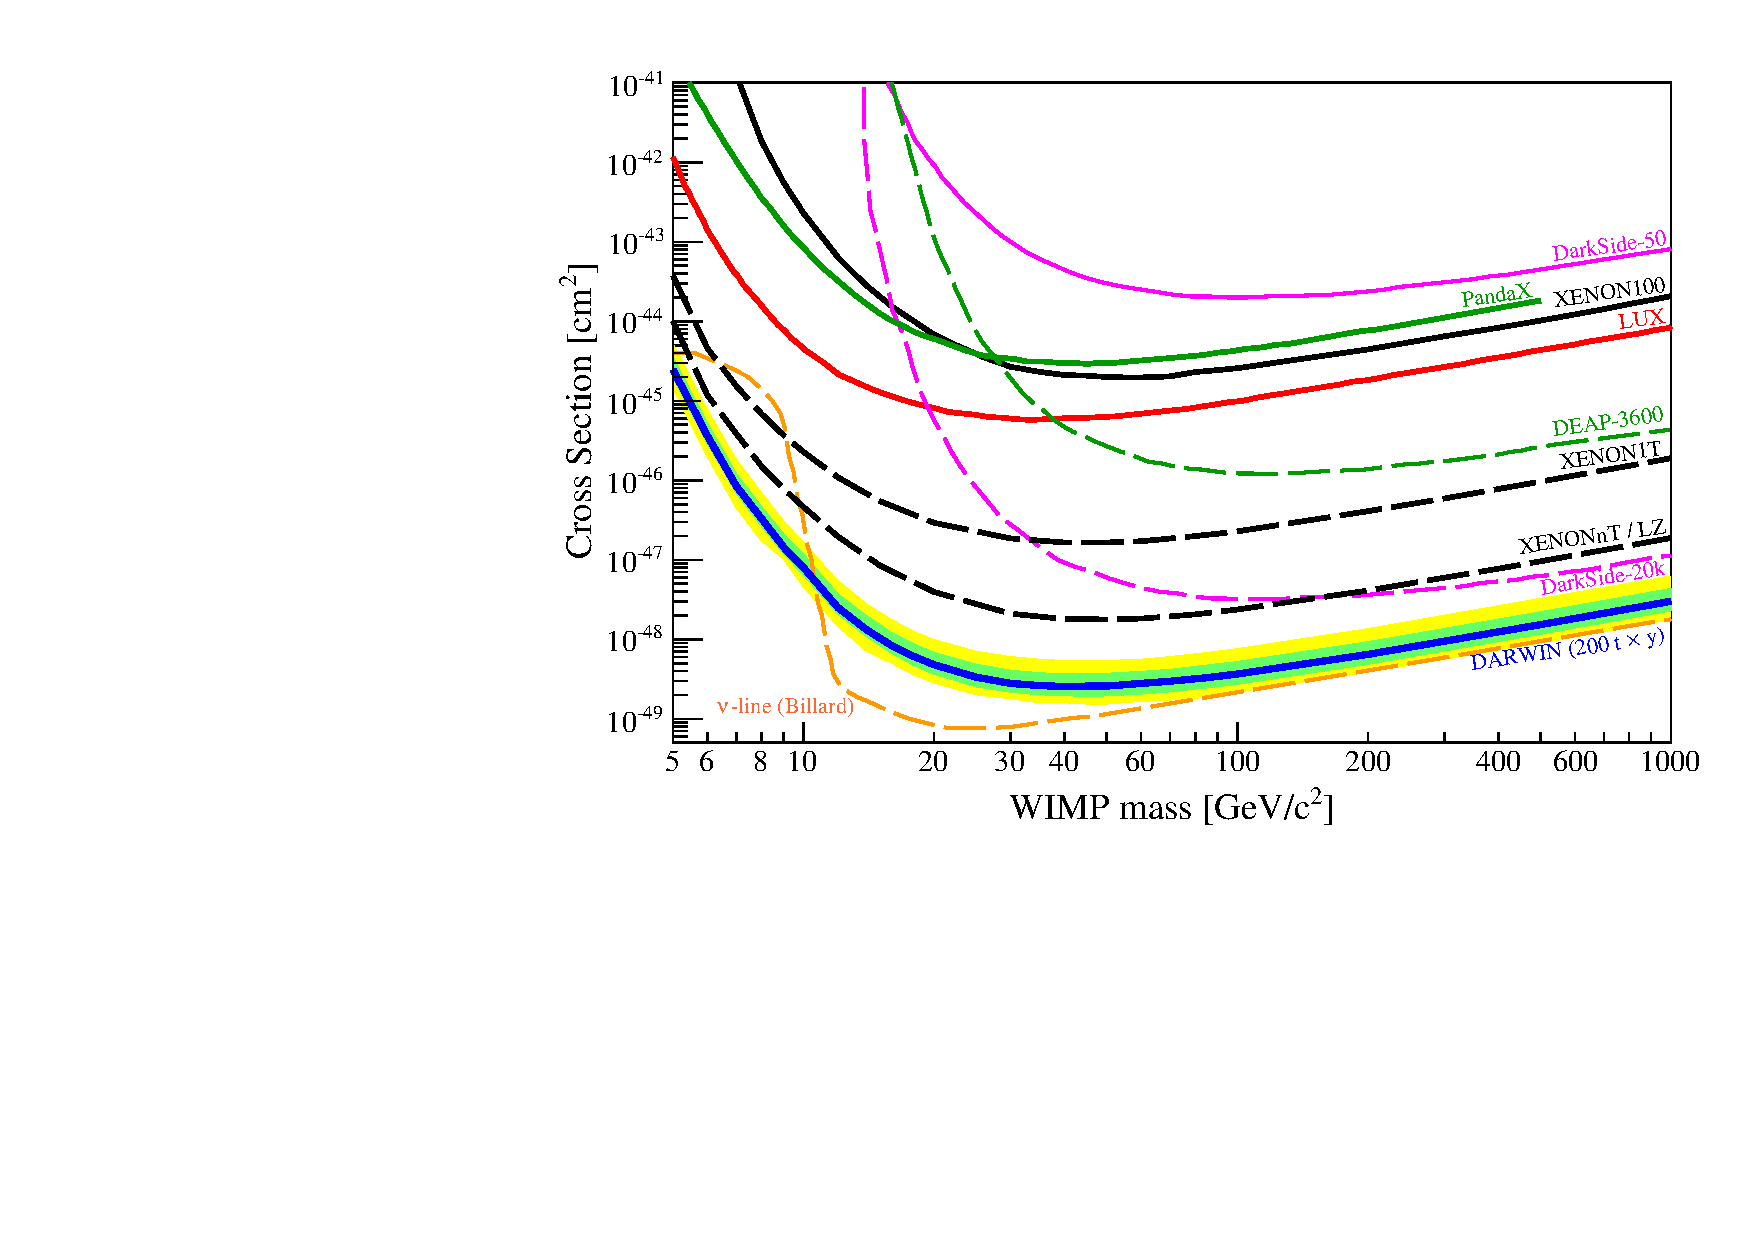
\includegraphics[width=0.8\textwidth]{figures/concl/darwin_sens}
    \caption{Expected sensitivity of the DARWIN experiment to the WIMP-nucleon scattering cross section. While an experiment with a greater sensitivity could be built, it would immediately encounter an unavoidable background from coherent neutrino-nucleus scattering, rendering a WIMP search extremely difficult. Figure from~\cite{Albers:2016jon}.}\label{fig:darwin_sens}
\end{figure}

The necessary \Rn~concentration necessary for DARWIN to reach this sensitivity is $\order{0.1}\1{mBq/tonne}$, a value two orders of magnitude lower than what was achieved for XENON1T and one order of magnitude lower than what will be required for XENONnT and LUX. Achieving this will require a combination of all of the above techniques.